% !TEX encoding = UTF-8
% !TEX TS-program = pdflatex
% !TEX root = ../CME-III-ARTICOLO.tex
% !TEX spellcheck = it-IT

%************************************************
\section*{Frammento Preparatorio alla Tesi}
\label{sec:frammento}
%************************************************

\begin{flushright}{\slshape
  …sì, per cui una chiesa barocca ha sotto di sé, \\
  accessibile, una chiesa romanica, \\
  sotto la chiesa romanica una basilica paleocristiana, \\
  poi si scende ancora e c’è il mitreo romano… \\
  Questa è Roma. \\
  Però, invece, apparentemente Roma è appunto atemporale, \\
  sembra non offrire nulla; \\
  e gli accessi sono segreti, alla vera realtà di Roma. \\
  Quindi corrisponde assai bene allo stadio opaco dell’infanzia e dell’adolescenza, \\
  quando si è in preda a questa cosa strana che è il voler scrivere…} \\ \medskip
    --- G. Agamben
\end{flushright}

\begin{description}
  \item[Year:] 2016
  \item[Instrumentation:] \emph {sax sopr. with pre-recorded environment}
  \item[Duration:] 7/9'
\end{description}

La scelta del luogo, dello spazio d'ascolto è il punto di partenza.
Partenza (dipartita), della stessa scrittura strumentale tradizionale.
Il brano, commissionato dall'\emph{Accademia Filarmonica Romana}, costituisce un primo studio
verso l'uso dello spazio come altro corpo musicale, altra costante della struttura
compositiva, in  relazione con lo strumento.
Anche quest'ultimo è praticato come luogo nel luogo, nel continuo scambio e
studio assieme allo strumentista.

\bigskip

Ciò che risulta essere oggetto di indagine nei confronti dello spazio riguarda
il suo rivelarsi e stratificarsi in un'altro ambiente d'ascolto, ovvero la sala da concerto.
Frammenti di una registrazione orchestrata e l'acustica architettonica della
chiesa di \emph{San luca e Martina} sono catturati tramite una  risposta tridimensionale all'impulso.
Ma non si tratta della registrazione quanto il ricordo  di uno spazio a portare
avanti il lavoro di scrittura: non un contenuto simbolico o di reale simulazione,
ma la possibilità di  un non-luogo, una non-voce che porta con se il ricordo offuscato degli eventi.

%************************************************
\section*{Traccia,ricordanza}
\label{sec:ricordanza}
%************************************************

Questo ricordo, la sua virtualizzazione, poggia sulle tecniche di registrazione
con tecnologia \emph{ambisonic} e sulla possibilità di registrazione tetraedrica
progettata da Michael Gerzon. Il microfono utilizzato, un \emph{Soundfield SPS200},
produce un segnale quadrifonico proveniente dalle rispettive capsule cardioidi posizionate
sui vertici di un tetraedro e denominato \emph{A-format}.

\begin{figure}
\centering
\subfloat[Tetraedro inscritto in un cubo]
{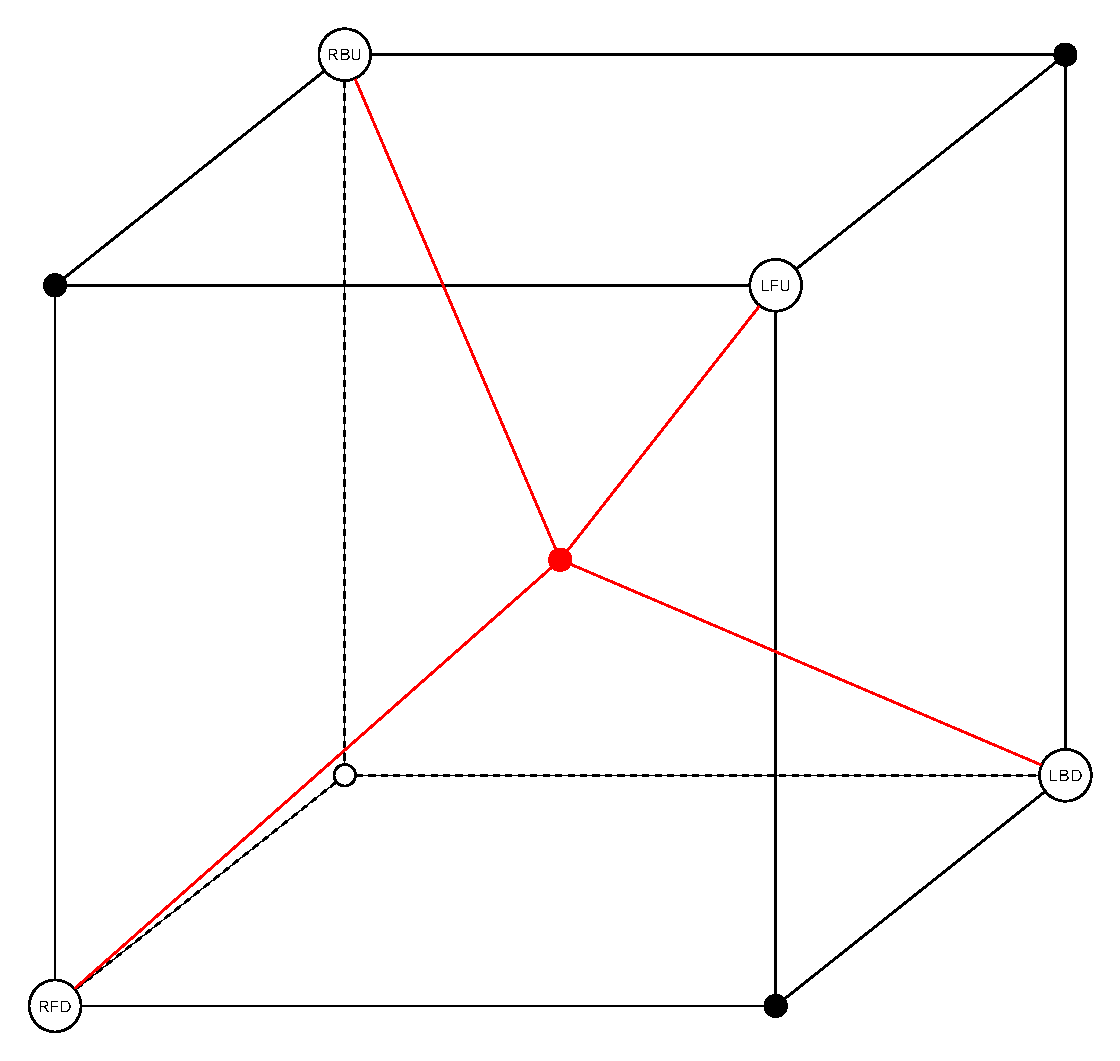
\includegraphics[width=.45\columnwidth]{tetrarec-cube}} \quad
\subfloat[Spazio Tetraedrico]
{\label{fig:tetracube}%
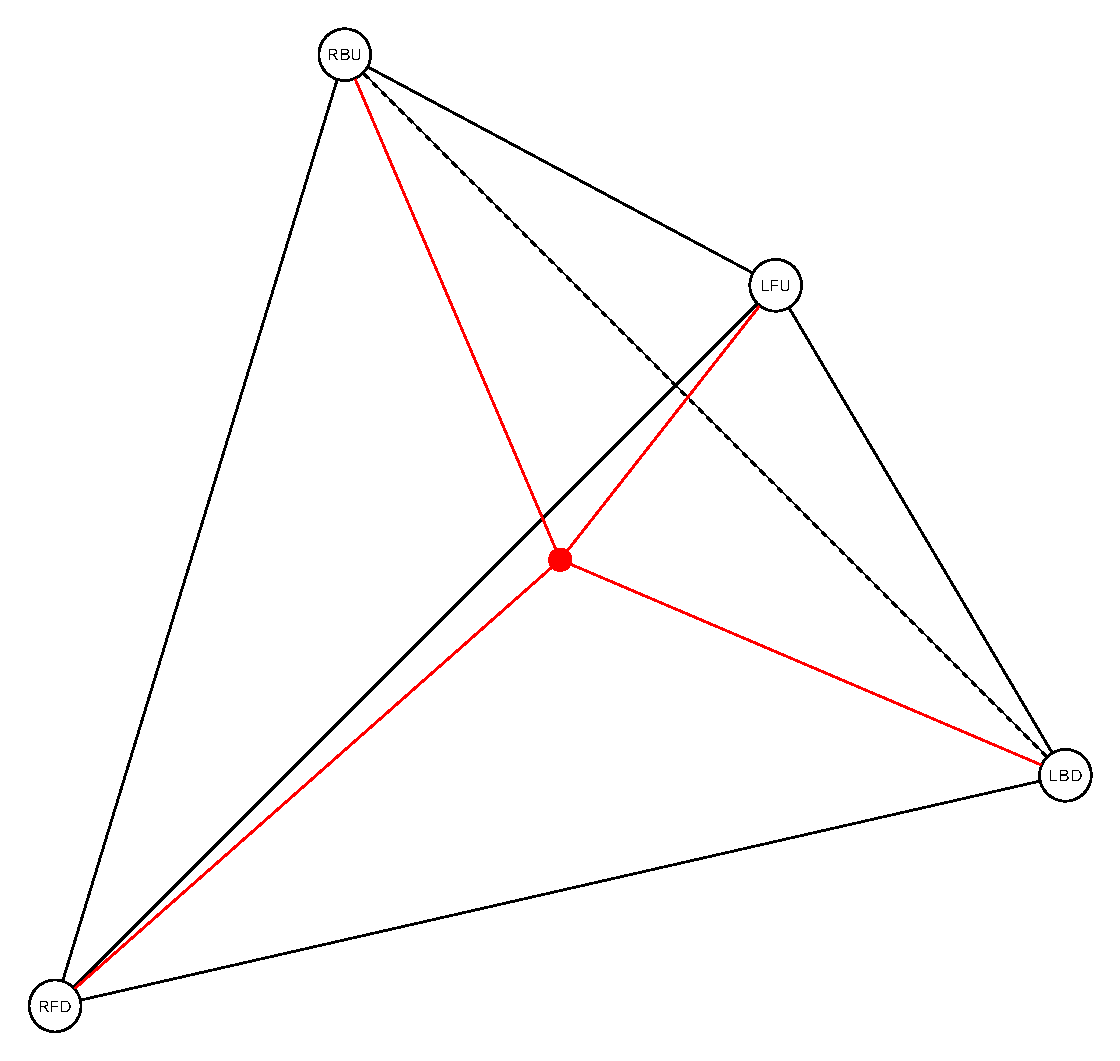
\includegraphics[width=.45\columnwidth]{tetrarec-tetrahedron}} \\
\caption[Spazio Tetraedrico]{Spazio Tetraedrico}
\label{fig:tetratetra}
\end{figure}

%5 parole ancora su Gerzon e ambisonic

La tecnologia descritta da Gerzon permette di descrivere un complesso sonoro
tridimensionale mediante armoniche sferiche denominato \emph{B-Format},
generato da una matrice di scomposizione dei quattro segnali del \emph{A-Format}.
Il \emph{B-Format}, composto da un'armonica di ordine \emph{zero} denominata $ W $
e tre vettori direzionali del \emph{primo} ordine denominati $ X, Y, Z $ può descrivere
vettori spaziali in tutte le dierezioni dello spazio sonoro.

Per la descrizione dello spazio sonoro di \emph{appunti} è stato utilizzato il
sistema di diffusione omnidirezionale \emph{S.T.ONE} in grado di riprodurre direttamente
segnali \emph{A-Format}.

Tracciare questa cartografia acustica della chiesa, tramite risposta all'impulso,
ha portato all'uso di 4 sweep esponeziali, dove agli angoli di un quadrato è
stato disposto il microfono soundfield. La scelta di forma è congiunta alla
disposizione di quattro altoparlanti tetraedrici nella sala da concerto, dove
lo strumentista si colloca tra i due altoparlanti anteriori.
La misurazione  tramite \emph{sweep esponenziale} è stata implementata su software
\emph{Pure Data}. Il segnale di chirop è stato riprodotto mediante altoparlante
tetraedrico \emph{S.T.ONE} e registrato attaverso il microfono \emph{SoundField SPS200}.

\begin{figure}
\centering
{\includegraphics[width=.95\columnwidth]{dolor}}
\caption[Pianta S. Luca]{Pianta S. Luca}
\label{fig:tetratetra}
\end{figure}

%************************************************
\section*{Struttura}
\label{sec:struttura}
%************************************************

Costruzione dell'environment


Tutto in ppppp l'idea  è di ricordanza dei suoni più che dell'effettivo sguardo “concreto”.

Fare i due schemi

Sono partito da due voci che instaurano un rapporto intervallare intorno alla sesta minore.

Questo rapporto intervallare modula sempre in corrispondenza di un centro
(della seconda voce) che è il sib. Mentre  la prima voce segue un processo poco
più complesso: mette in gioco la qualità dei battimenti.

(generati sia dallo spazio tramite convoluzione sia dal sassofono).
La qualità del battimento è fondamentale e questa trasformazione entro la seconda
minore è sia gioco intorno al polo in quell'istante sia “interruttore” per
lo spostamento del polo.

\begin{figure}
\centering
{\includegraphics[width=.95\columnwidth]{dolor}}
\caption[Appunti Partitura]{Appunti Partitura}
\label{fig:tetratetra}
\end{figure}

1)Struttura formale iniziale (astratta):
Anche qui la struttura la divido in 7 parti ma il discorso è sempre duale (A/B),
tra suoni tenuti fino alla perdita di forma e suono che costruisce un senso di fraseggio.
A= zona informale, corone
B=Voce, volontà di fraseggio

in realtà questa scelta di discendenza non viene praticata correttamente.
Ho seguito la mia esperienza per arrivare ad un fine: non rendere subito questa
idea di spostamento delle componenti frequenziali verso il basso.

1)Struttura iniziale (astratta):
Struttura è divisa in 7 blocchi ma il discorso è sempre duale (A/B), tra suoni
tenuti fino alla perdita di forma e suono che costruisce un senso di fraseggio.

A= zona informale, corone
B=Voce, volontà di fraseggio

Tutto in ppppp l'idea  è di ricordanza dei suoni più che dell'effettivo sguardo “concreto”.
Per semplificare invece il discorso riverbero della chiesa, quello che avviene è
uno stazionamento di determinate frequenze che tramite i feedback che costituiscono
il riverbero aumentano di ampiezza. L'aumento di ampiezza corrisponde anche ad un loro
decadimento più lento e questo determina anche la scelta delle frequenze successive a
quella in risonanza con la chiesa: questo per arrivare  battimento/modulazionie di
ampiezza data dalla stanza stessa (quasi un squarcio del riverbero)

%
% \subsection{Mane}
% \lipsum[2]
%
% \subsection{Tekel}
% \lipsum[3]
%
% \subsection{Fares}
% \lipsum[4-5]
